\section{Timeline}


\begin{itemize}
\item ComCam will go on the TMA next month
	\begin{itemize}
	\item We will have images, potentially on Sky images, before year end.
	\item We will have loads of calibration data
	\end{itemize}
\item We should be able to process ComCam images at SLAC in June.
	\begin{itemize}
	\item Would be nice to process all the BOT data
	\end{itemize}
\item Officially engineering first light is Jan 2023 (likely a little later)
	\begin{itemize}
	\item Then we need OGA racks etc.
	\item We will still be getting lots of engineering data from the real camera !
	\end{itemize}
\end{itemize}

The USDF timeline is in \citeds{RTN-021} the high level milestone chart is duplicated in\figref{fig:usdfplan} here.


\begin{figure}
\begin{centering}
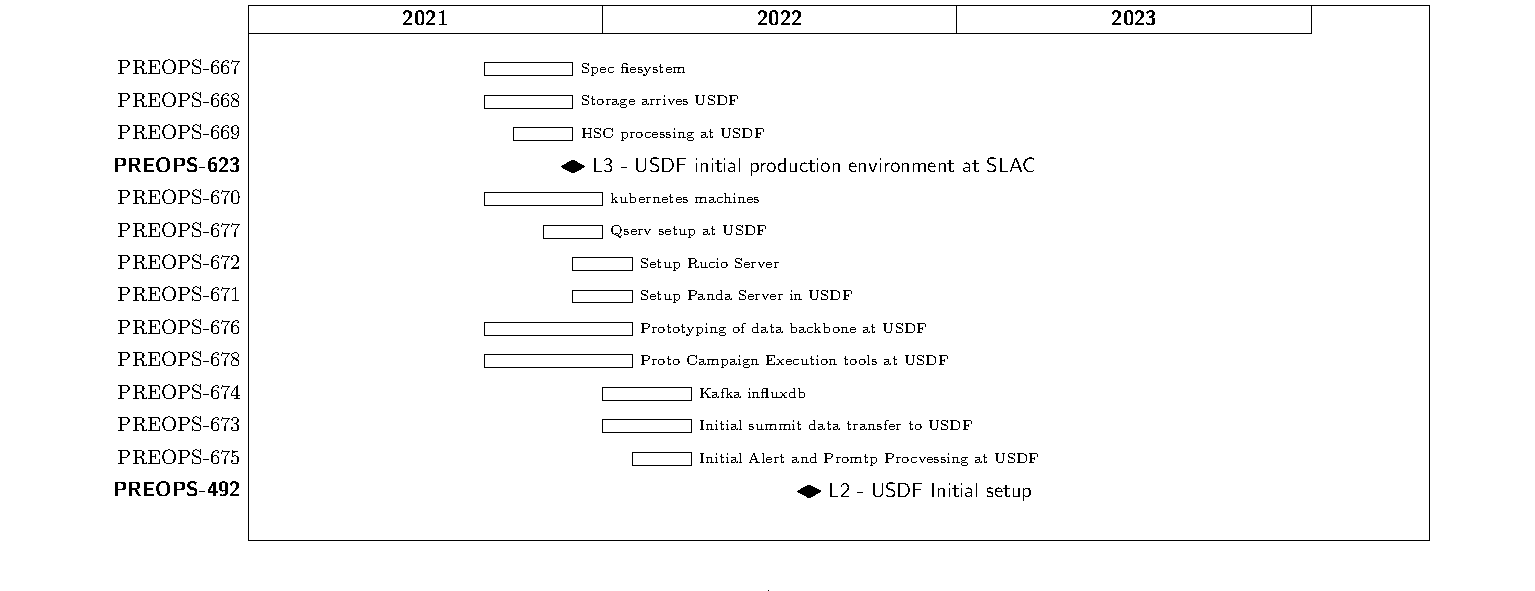
\includegraphics[width=0.9\textwidth]{USDFplan}
	\caption{USDF buildup plan from \citeds{RTN-021}\label{fig:usdfplan}}
\end{centering}
\end{figure}

The big question right now is {\em When can we start multi site testing with PanDA/Rucio ..
IDF, SLAC, FRdF all run PanDA \ldots}.

We need to build up tests for distributed processing RUCIO PanDA, which has started!


We need to make Jira Epics and capture decisions in technotes.

As always KISS!\footnote{Yes it is in the glossary.}


